% !TEX program = pdflatex
\documentclass[letterpaper,12pt]{article}
\usepackage[spanish,mexico]{babel}
\usepackage[T1]{fontenc}
\usepackage{lmodern}
\usepackage{amsmath,amssymb}
\usepackage{graphicx,float,subcaption,xcolor,array,booktabs,tabularx,ragged2e}
\usepackage{tikz}
\usetikzlibrary{arrows.meta,positioning,shapes.geometric,calc}
\usepackage{listings}
\usepackage[left=25mm,right=25mm,top=35mm,bottom=30mm,headheight=15pt]{geometry}
\usepackage{parskip,fancyhdr}
\usepackage{hyperref}

\graphicspath{{img/}{portada_img/}}
\newcommand{\materia}{Laboratorio de Organización y Arquitectura de Computadoras}
\pagestyle{fancy}
\fancyhf{}
\fancyhead[R]{\textsc{\materia}}
\fancyfoot[C]{\thepage}
\renewcommand{\headrulewidth}{0.8pt}
\hypersetup{colorlinks=true,linkcolor=blue,urlcolor=cyan}

\definecolor{codebg}{rgb}{0.96,0.96,0.96}
\definecolor{keyword}{rgb}{0.0,0.2,0.6}
\definecolor{comment}{rgb}{0.25,0.5,0.35}
\definecolor{codegray}{rgb}{0.5,0.5,0.5}
\lstdefinestyle{estiloVHDL}{
  language=VHDL,basicstyle=\ttfamily\scriptsize,
  backgroundcolor=\color{codebg},commentstyle=\color{comment}\itshape,
  keywordstyle=\color{keyword}\bfseries,numbers=left,
  numberstyle=\tiny\color{codegray},frame=single,breaklines=true,
  literate={á}{{\'a}}1 {é}{{\'e}}1 {í}{{\'i}}1 {ó}{{\'o}}1 {ú}{{\'u}}1 {ñ}{{\~n}}1 {←}{{$\leftarrow$}}1,
  keepspaces=true,showstringspaces=false,tabsize=2,
  morekeywords={library,use,all,entity,is,port,in,out,architecture,of,begin,end,signal,constant,process,if,then,else,elsif,case,when,others,std_logic,std_logic_vector}
}
\lstdefinestyle{mif}{style=estiloVHDL,language={},morecomment=[l]{--},numbers=none}
\lstdefinestyle{asm}{style=estiloVHDL,language={},morecomment=[l]{;},numbers=none}
\lstdefinestyle{pseudo}{style=estiloVHDL,language=C,morecomment=[l]{//},numbers=none}

\newcommand{\hx}[1]{\texttt{#1}}
\newcolumntype{Y}{>{\RaggedRight\arraybackslash}X}
\renewcommand{\lstlistingname}{Código}
\setlength{\emergencystretch}{2em}

\begin{document}
\thispagestyle{empty} % Sin encabezado ni pie en la portada

% --- ENCABEZADO DE PORTADA (TABLA DE 3 COLUMNAS) ---
\begin{center}
    % La tabla usa 'm' para centrar verticalmente las imágenes y el texto
    \begin{tabular}{m{0.15\textwidth} m{0.60\textwidth} m{0.15\textwidth}}
        % Logo Izquierdo (UNAM)
        
\includegraphics[width=2cm]{portada_img/escudounam_negro.jpg} & 
        
        % Título Central
        \centering\Huge\textbf{Universidad Nacional Autónoma de México} &
        
        % Logo Derecho (Facultad)
        \raggedleft
\includegraphics[width=2cm]{portada_img/escudofi_negro.jpg}
    \end{tabular}
\end{center}

\vspace{0.3cm}

% --- INFORMACIÓN DEL REPORTE ---
\begin{center}
    {\LARGE \textbf{Facultad de Ingeniería}}\\[1cm]

    {\LARGE \textbf{Laboratorio de Arquitectura y Organización de Computadoras}} \\[1cm]

	{\LARGE Grupo: 07 - Semestre: 2027-1} \\[1cm]
    
    {\LARGE \textbf{Reporte Práctica 7 Pt 2.}}\\[0.5cm]
    {\LARGE Procesador CISC 68HC11}\\[1cm]

    {\Large \textbf{Fecha de Entrega}}\\[0.2cm]
    {\Large 20 de Noviembre del 2026} \\[1cm]

    {\LARGE \textbf{Profesor}}\\[0.2cm]
    {\Large Ing. Julio Cesar Cruz Estrada}\\[1cm]
    
    {\LARGE \textbf{Integrantes:}}\\[0.2cm]
    {\Large Espinoza Matamoros Percival Ulises}\\[0.5cm]
    {\Large Montiel Juárez Oscar Iván}\\[0.5cm]
    {\Large Veraza García Amy Valentina}\\[0.5cm]

\end{center}

\newpage

%==============================================================
\section{Objetivo}

Obtener el mayor de cinco números de 8 bits sin signo y guardarlo en \texttt{Res}, mediante un programa para el procesador CISC 68HC11 y la implementación del salto condicional \texttt{JAE}.

%==============================================================
\section{Desarrollo}

Se agregó \texttt{JAE} en \texttt{Secuenciador/memory.vhd} y se cargaron el programa y los datos en RAM mediante \texttt{mem\_content.mif}. Se reutilizaron las instrucciones de carga, comparación y almacenamiento del proyecto de Quartus.

\subsection{Lógica para obtener el número mayor}

$A$ conserva el mayor encontrado y $B$ recibe el siguiente elemento. Se carga $L[0]$ en $A$ y se compara con los otros cuatro valores: si $B>A$, se actualiza $A$; al terminar, se copia a \texttt{Res}.

\begin{lstlisting}[style=pseudo,caption={Lógica del algoritmo para una lista de cinco números.},label={lst:logica}]
L = [0x05, 0x09, 0x01, 0x02, 0x06];
mayor = L[0];
for (i = 1; i < 5; i++) {
    if (L[i] > mayor) {
        mayor = L[i];
    }
}
Res = mayor;
\end{lstlisting}

En ensamblador, el ciclo del Código~\ref{lst:logica} se implementó con cuatro bloques consecutivos, sin contador de iteraciones. Los datos se representan en hexadecimal y se interpretan sin signo, de 0 a 255.

\subsection{Instrucciones utilizadas}

La Tabla~\ref{tab:instrucciones} resume las instrucciones del programa. La única rutina nueva fue \texttt{JAE}, con el opcode \hx{7C}.

\begin{table}[H]
\centering
\small
\caption{Instrucciones empleadas para encontrar y almacenar el mayor.}
\label{tab:instrucciones}
\begin{tabularx}{\linewidth}{c l c Y}
\toprule
Opcode & Instrucción & Modo & Función en el programa \\
\midrule
\hx{96} & \texttt{LDAA} & EXT & Cargar el primer elemento en $A$ o actualizar el mayor. \\
\hx{F6} & \texttt{LDAB} & EXT & Cargar el siguiente elemento de la lista en $B$. \\
\hx{1C} & \texttt{CMP} & INH & Calcular $A-B$ para actualizar las banderas, sin modificar los acumuladores. \\
\hx{7C} & \texttt{JAE} & EXT & Saltar si $A\geq B$, omitiendo la actualización de $A$. \\
\hx{A7} & \texttt{STAA} & EXT & Guardar el mayor de $A$ en \texttt{Res}. \\
\hx{7E} & \texttt{JMP} & EXT & Mantener el programa en un ciclo final. \\
\bottomrule
\end{tabularx}
\end{table}

Cada bloque ejecuta \texttt{LDAB}, \texttt{CMP} y \texttt{JAE}. Si $A\geq B$, el salto omite el \texttt{LDAA} siguiente; si $A<B$, esa carga actualiza el mayor.

\subsection{Comparación y bandera de acarreo}

\texttt{CMP} calcula $A-B$ y actualiza las banderas sin modificar los acumuladores. En esta UPA, el bit adicional de la resta determina $C$:
\[
C=\begin{cases}
1, & A<B,\\
0, & A\geq B.
\end{cases}
\]

Por ello, \texttt{JAE} toma el salto cuando $C=0$. Se usa $C$ porque la comparación es sin signo; $N$ por sí sola no determina el orden en todo el intervalo de 8 bits. Las señales con prefijo \texttt{n} se habilitan en bajo; las demás señales indicadas en la Tabla~\ref{tab:cmp-control} valen 1.

\begin{table}[H]
\centering
\scriptsize
\caption{Señales de control utilizadas por \texttt{CMP}.}
\label{tab:cmp-control}
\begin{tabularx}{\linewidth}{c Y Y}
\toprule
Estado & Señales & Función \\
\midrule
\hx{1C0} & EA1, EA0, EB1, EB0, UPA5, UPA0, selmux, ACCSEC & EA y EB conectan los acumuladores a la UPA. UPA0 selecciona $A$ y $B$; UPA5 selecciona la resta. selmux y ACCSEC fijan $C_{in}=1$ para obtener $A-B$. \\
\hx{1C1} & nOEUPA=0, nDUPA=0, CC, CN, CV, CZ & Se conserva la salida registrada de la UPA y se cargan las banderas. nWA=nWB=1 evitan modificar los acumuladores. \\
\hx{1C2} & nEPC2=0, nCBD=0 & Se prepara la siguiente búsqueda y se regresa a \hx{009}. \\
\bottomrule
\end{tabularx}
\end{table}

\subsection{Implementación de JAE}

Se copiaron las seis microinstrucciones de \texttt{JE} a \hx{7C0}--\hx{7C5}, conservando las transferencias y cambiando la condición y la liga en \hx{7C3}. MAP dirige el opcode \hx{7C} a \hx{7C0}; después se leen los dos bytes del destino, primero el alto y luego el bajo, en RA.

La palabra de microprograma tiene 98 bits: 20 de secuenciamiento y 78 de control. En \hx{7C3} se definieron estos campos:
\[
\underbrace{\texttt{10000}}_{\text{prueba de }C}\;
\underbrace{\texttt{1}}_{VF}\;
\underbrace{\texttt{01}}_{\text{salto condicional}}\;
\underbrace{\texttt{0111\,1100\,0101}}_{\text{liga }\hx{7C5}}.
\]

El secuenciador evalúa $CC_{\text{sec}}=\overline{C\oplus VF}$. Con instrucción \texttt{01}, carga la liga si hay coincidencia; de lo contrario, continúa al siguiente microestado:
\begin{itemize}
  \item $C=1$ ($A<B$): salta a \hx{7C5}, omite la carga del PC y continúa con el \texttt{LDAA} que actualiza $A$.
  \item $C=0$ ($A\geq B$): ejecuta \hx{7C4}, carga $\text{PC}\leftarrow\text{RA}$ y omite la actualización de $A$.
\end{itemize}

Así, saltar internamente a \hx{7C5} evita tomar el salto del programa. $CC_{\text{sec}}$ es la condición del secuenciador; la señal \texttt{CC} de \texttt{CMP} habilita la carga de la bandera de acarreo.

\begin{table}[H]
\centering
\scriptsize
\caption{Transferencias y señales de control de \texttt{JAE} (EXT).}
\label{tab:jae-control}
\begin{tabularx}{\linewidth}{c Y Y}
\toprule
Estado & Transferencia & Señales y motivo \\
\midrule
\hx{7C0} & Reg. Dir $\leftarrow$ PC & nEPC2=0 habilita el PC en el bus de direcciones; nCBD=0 captura su valor. \\
\hx{7C1} & RA$_{\text{ALTA}}\leftarrow$ Mem; PC $\leftarrow$ PC$+1$ & nAS=0 y nRW=1 leen memoria. BD=1, nERA1=0 y RA2=1 cargan el byte alto. PC0=1 incrementa el PC. \\
\hx{7C2} & Reg. Dir $\leftarrow$ PC & nEPC2=0 y nCBD=0 preparan la dirección del segundo byte. \\
\hx{7C3} & RA$_{\text{BAJA}}\leftarrow$ Mem; PC $\leftarrow$ PC$+1$; prueba de $C$ & nAS=0 y nRW=1 leen memoria. BD=0, nERA0=0 y RA1=RA0=1 cargan el byte bajo. PC0=1 incrementa el PC. \\
\hx{7C4} & PC $\leftarrow$ RA, sólo si $C=0$ & nERA1=nERA0=0 habilitan RA en ambos buses. nEPC1=nEPC0=0 y PC2=PC0=1 cargan los 16 bits del PC. \\
\hx{7C5} & Reg. Dir $\leftarrow$ PC & nEPC2=0 y nCBD=0 preparan la búsqueda de la siguiente instrucción. \\
\bottomrule
\end{tabularx}
\end{table}

\hx{7C4} conserva la prueba de interrupciones \texttt{01111/1/11/000}; \hx{7C5} usa \texttt{11000/0/01/009} para volver a la búsqueda. El Código~\ref{lst:jae} muestra las palabras agregadas antes del \texttt{else} final de \texttt{memory.vhd}.

\begin{lstlisting}[style=estiloVHDL,caption={Microprograma agregado para JAE con opcode 7C.},label={lst:jae}]
-- JAE (EXT): salta si A >= B, es decir, C = 0
elsif(dir= X"7C0") then data <=
  "00000" & "0" & "00" & "000000000000" &
  "100100100000000000110111000011100011100001100001111110000000000000000000000010";
elsif(dir= X"7C1") then data <=
  "00000" & "0" & "00" & "000000000000" &
  "100100100000000000110111000010110011100011100111111011000000000000000000000010";
elsif(dir= X"7C2") then data <=
  "00000" & "0" & "00" & "000000000000" &
  "100100100000000000110111000011100011100001100001111110000000000000000000000010";
elsif(dir= X"7C3") then data <=
  "10000" & "1" & "01" & "011111000101" &
  "100100100000000000110111000011001111100011100111111010000000000000000000000010";
elsif(dir= X"7C4") then data <=
  "01111" & "1" & "11" & "000000000000" &
  "100100100000000000110111000010000011100010010111111110000000000000000000000010";
elsif(dir= X"7C5") then data <=
  "11000" & "0" & "01" & "000000001001" &
  "100100100000000000110111000011100011100001100001111110000000000000000000000010";
\end{lstlisting}

\subsection{Programa y distribución de la RAM}

El programa ocupa las posiciones decimales 0--48, la lista las posiciones 49--53 (\hx{0031}--\hx{0035}) y \texttt{Res} la posición 54 (\hx{0036}). Cada \texttt{JAE} apunta al siguiente bloque o al almacenamiento final. Las direcciones del Código~\ref{lst:ensamblador} están en hexadecimal.

\begin{lstlisting}[style=asm,caption={Programa en ensamblador para obtener el mayor de cinco elementos.},label={lst:ensamblador}]
Dir.   Bytes      Instruccion
0000   96 00 31   LDAA $0031    ; A = L[0]
0003   F6 00 32   LDAB $0032    ; B = L[1]
0006   1C         CMP           ; comparar A-B
0007   7C 00 0D   JAE  $000D    ; conservar A si A >= B
000A   96 00 32   LDAA $0032    ; actualizar el mayor
000D   F6 00 33   LDAB $0033    ; B = L[2]
0010   1C         CMP
0011   7C 00 17   JAE  $0017
0014   96 00 33   LDAA $0033
0017   F6 00 34   LDAB $0034    ; B = L[3]
001A   1C         CMP
001B   7C 00 21   JAE  $0021
001E   96 00 34   LDAA $0034
0021   F6 00 35   LDAB $0035    ; B = L[4]
0024   1C         CMP
0025   7C 00 2B   JAE  $002B
0028   96 00 35   LDAA $0035
002B   A7 00 36   STAA $0036    ; Res = A
002E   7E 00 2E   JMP  $002E    ; ciclo final
\end{lstlisting}

\texttt{STAA \$0036} sobrescribe \texttt{Res} con $A$: en \hx{A74}, nERA2=0 y nCBD=0 cargan la dirección desde RA; en \hx{A75}, EA0=1 coloca el dato en el bus y nAS=nRW=0 permiten escribirlo en RAM. Después, \texttt{JMP \$002E} repite el salto sin modificar el resultado y evita ejecutar la lista como instrucciones.

En \texttt{mem\_content.mif} se usan \texttt{WIDTH=8}, \texttt{DEPTH=256}, \texttt{ADDRESS\_RADIX=UNS} y \texttt{DATA\_RADIX=HEX}. Las posiciones 0--48 contienen los bytes del Código~\ref{lst:ensamblador}; el fragmento siguiente completa los datos y el relleno de la RAM:

\begin{lstlisting}[style=mif,caption={Datos y relleno final del archivo MIF para el primer ejemplo.},label={lst:datos1}]
    49 : 05; -- L[0]
    50 : 09; -- L[1]
    51 : 01; -- L[2]
    52 : 02; -- L[3]
    53 : 06; -- L[4]
    54 : 00; -- Res: valor inicial
    [55..255] : 00;
END;
\end{lstlisting}

%==============================================================
\section{Simulación}

Se simuló en Quartus mediante ModelSim con un reloj de 10\,ns, \texttt{RESET=1} e \texttt{IRQn=XIRQn=1}. Se observaron los acumuladores, RA, PC, \texttt{Edo\_Pres} y \texttt{csnn}. Se amplió la duración para incluir la última comparación, la escritura y el ciclo final; las transferencias se reflejan un ciclo después del estado que genera sus señales.

\subsection{Ejemplo 1: lista [05,09,01,02,06]}

\begin{figure}[H]
\centering
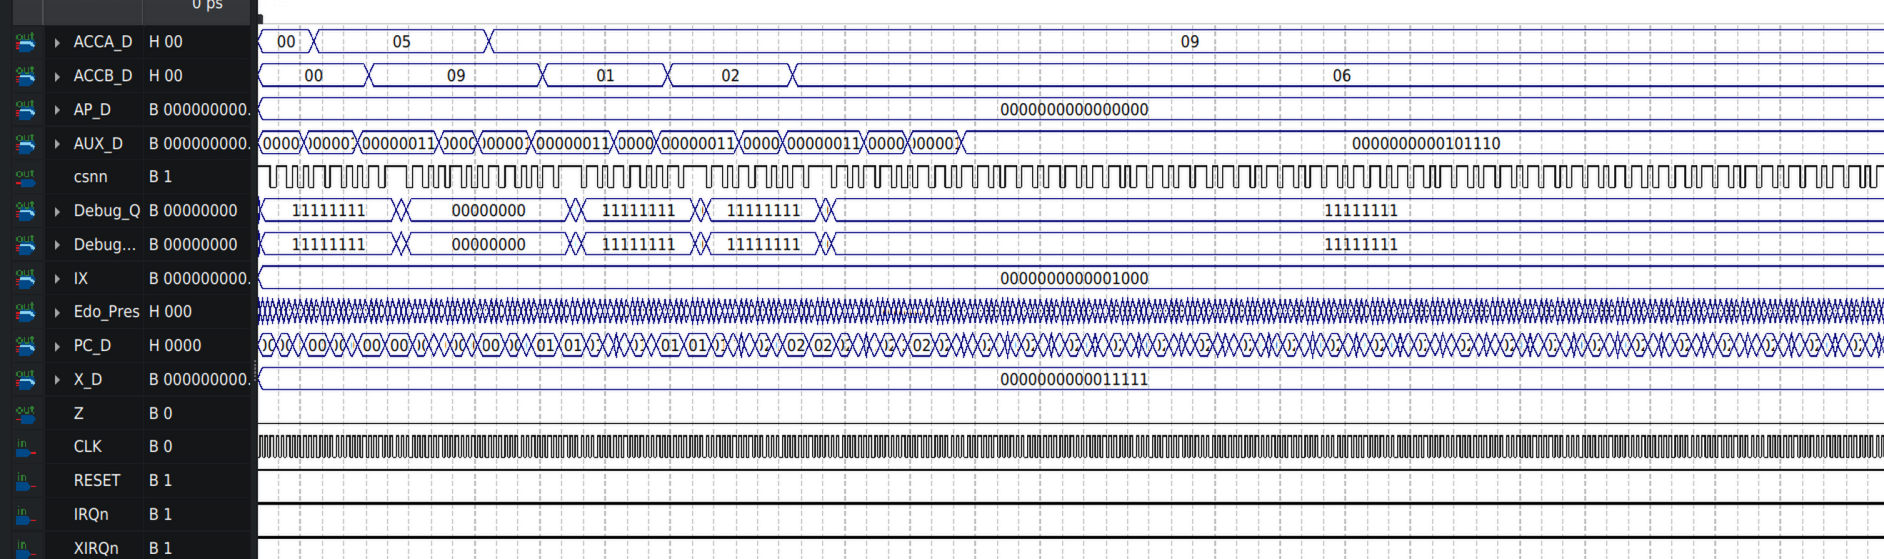
\includegraphics[width=\linewidth]{ejemplo_1.png}
\caption{Simulación de la búsqueda del mayor para la lista [05,09,01,02,06].}
\label{fig:ejemplo1}
\end{figure}

En la Figura~\ref{fig:ejemplo1}, $A$ carga \hx{05} y cambia a \hx{09} al compararse con el segundo elemento. Después conserva \hx{09} frente a \hx{01}, \hx{02} y \hx{06}, como resume la Tabla~\ref{tab:ejemplo1}. Finalmente, \texttt{STAA} guarda \hx{09} en \texttt{Res}.

\begin{table}[H]
\centering
\small
\caption{Comparaciones realizadas en el primer ejemplo.}
\label{tab:ejemplo1}
\begin{tabularx}{\linewidth}{c c c Y c}
\toprule
$A$ antes & $B$ & $C$ & Acción & $A$ después \\
\midrule
\hx{05} & \hx{09} & 1 & Actualizar $A$. & \hx{09} \\
\hx{09} & \hx{01} & 0 & Conservar $A$. & \hx{09} \\
\hx{09} & \hx{02} & 0 & Conservar $A$. & \hx{09} \\
\hx{09} & \hx{06} & 0 & Conservar $A$. & \hx{09} \\
\bottomrule
\end{tabularx}
\end{table}

\subsection{Ejemplo 2: lista [03,02,09,0C,0B]}

Se cambiaron únicamente los cinco datos de la lista, conservando el programa y las direcciones.

\begin{figure}[H]
\centering
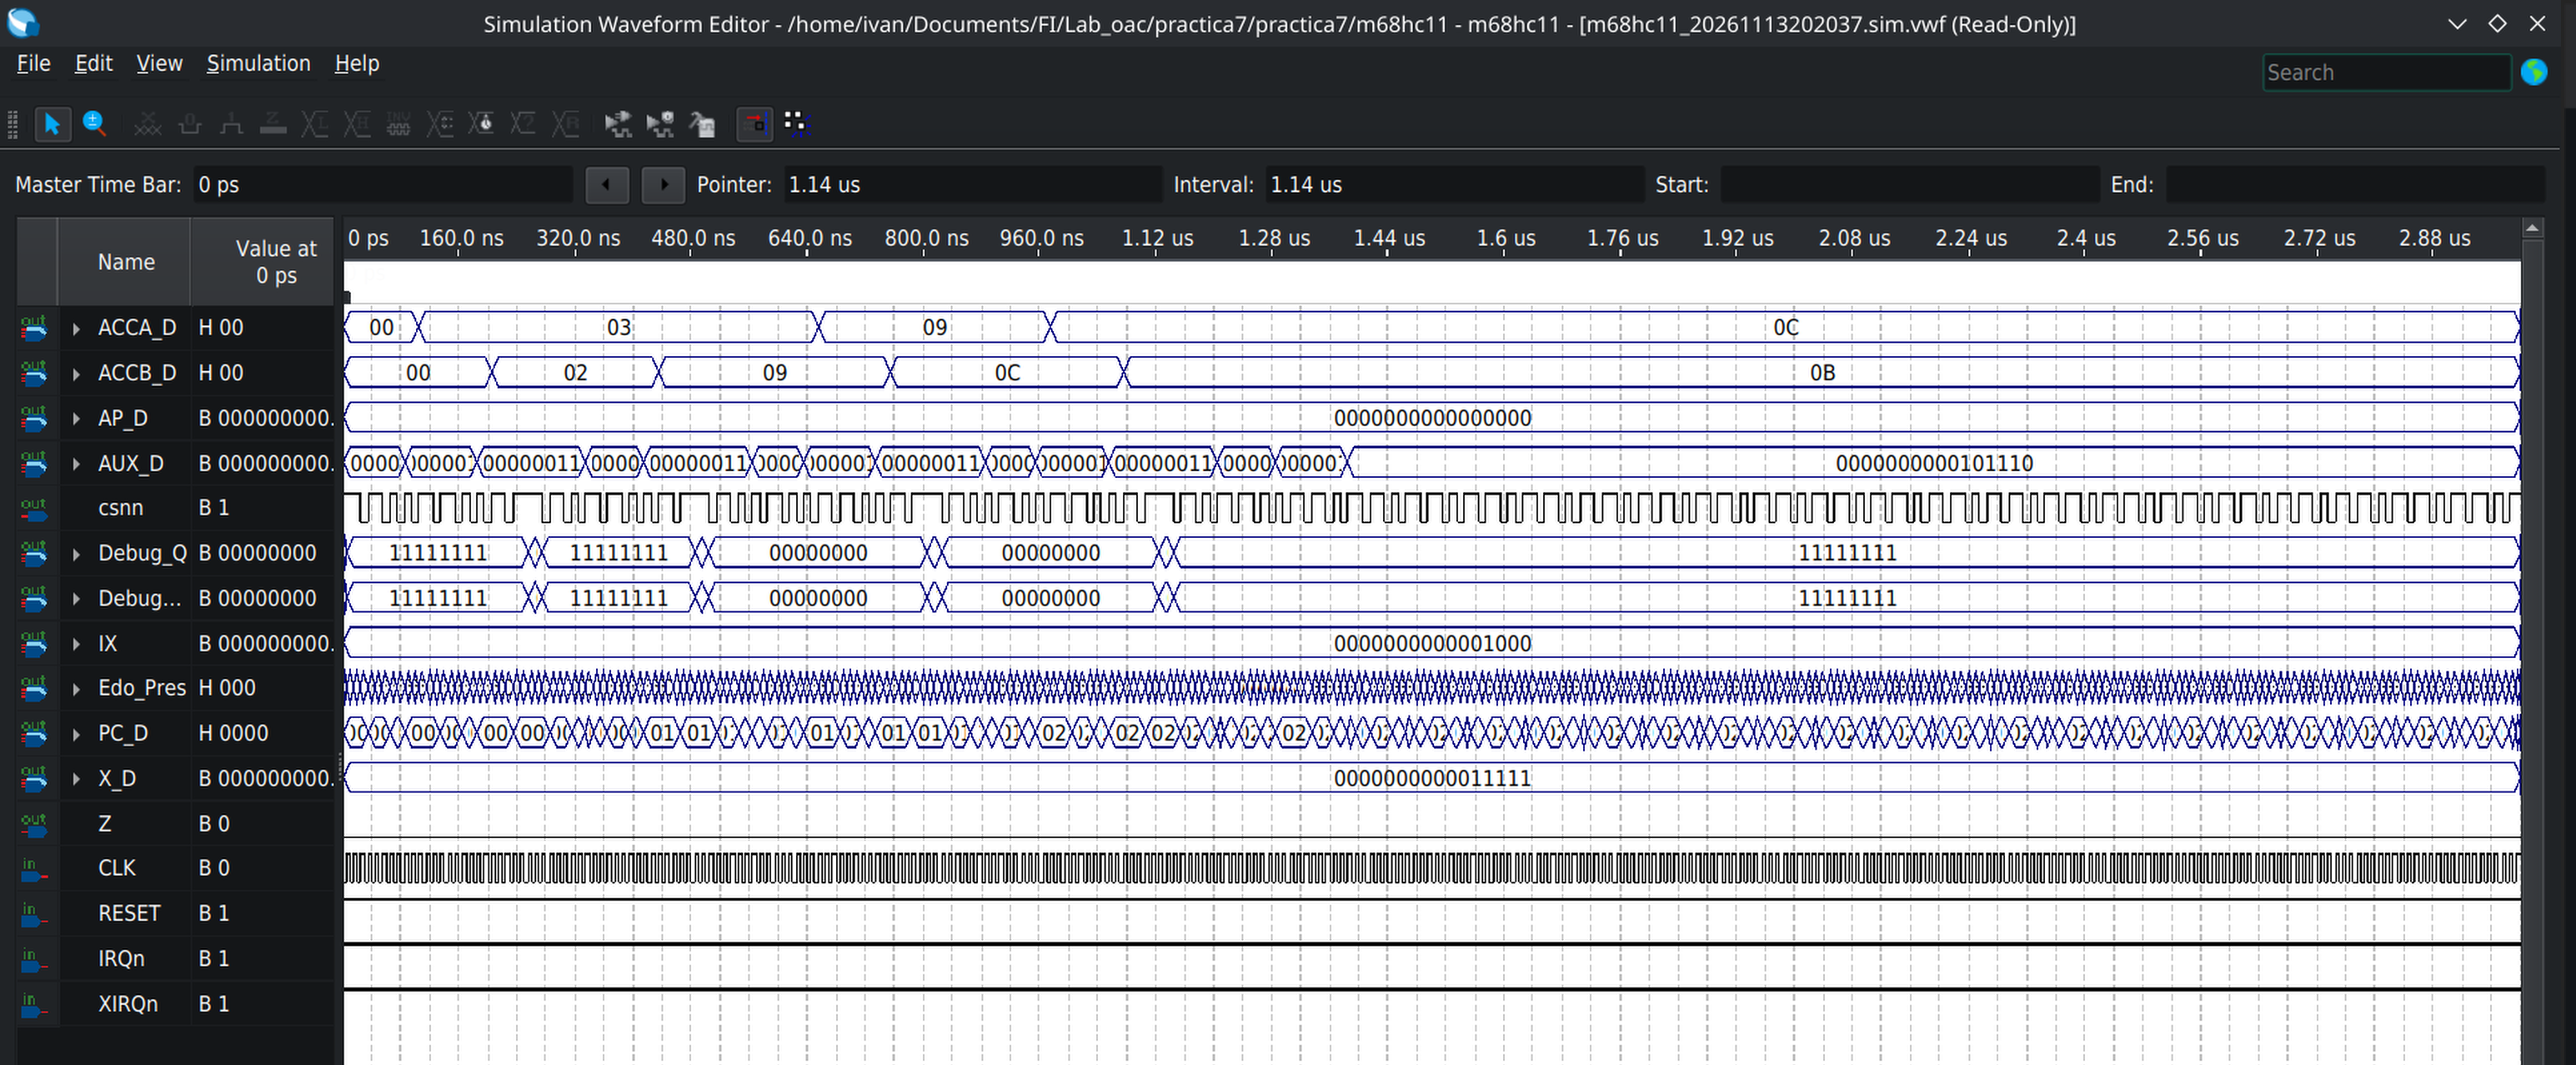
\includegraphics[width=\linewidth]{ejemplo_2.png}
\caption{Simulación de la búsqueda del mayor para la lista [03,02,09,0C,0B].}
\label{fig:ejemplo2}
\end{figure}

En la Figura~\ref{fig:ejemplo2}, $A$ conserva \hx{03} frente a \hx{02}; luego se actualiza a \hx{09} y a \hx{0C}. La última comparación con \hx{0B} conserva \hx{0C}, que se guarda en \texttt{Res}. La Tabla~\ref{tab:ejemplo2} muestra las cuatro decisiones.

\begin{table}[H]
\centering
\small
\caption{Comparaciones realizadas en el segundo ejemplo.}
\label{tab:ejemplo2}
\begin{tabularx}{\linewidth}{c c c Y c}
\toprule
$A$ antes & $B$ & $C$ & Acción & $A$ después \\
\midrule
\hx{03} & \hx{02} & 0 & Conservar $A$. & \hx{03} \\
\hx{03} & \hx{09} & 1 & Actualizar $A$. & \hx{09} \\
\hx{09} & \hx{0C} & 1 & Actualizar $A$. & \hx{0C} \\
\hx{0C} & \hx{0B} & 0 & Conservar $A$. & \hx{0C} \\
\bottomrule
\end{tabularx}
\end{table}

\subsection{Verificación del almacenamiento}

Las capturas muestran el mayor en $A$; \texttt{Res} es el contenido de RAM en \hx{0036}. Su escritura se verifica en \hx{A75}, con nAS=nRW=0, dirección \hx{0036} y el dato de $A$. \texttt{csnn} por sí sola no distingue lectura de escritura.

Después, el \texttt{JMP} final carga RA con \hx{002E}, visible como \texttt{0000000000101110} en \texttt{AUX\_D}. El PC repite \hx{002F}, \hx{0030}, \hx{0031} y \hx{002E}; \hx{0031} es transitorio y la lista no se ejecuta. El resultado permanece en RAM: \hx{09} para la primera prueba y \hx{0C} para la segunda.

%==============================================================
\clearpage
\section{Conclusión}

\paragraph{Percival Ulises Espinoza Matamoros.} En esta práctica pude relacionar la búsqueda del mayor de una lista con las instrucciones que ejecuta el procesador. La implementación de \texttt{JAE} me permitió comprender cómo las banderas y el secuenciador deciden si se conserva o se actualiza un dato. Al probar dos listas, observé que el programa obtiene distintos resultados sin cambiar sus instrucciones.

\paragraph{Oscar Iván Montiel Juárez.} En esta práctica entendimos de manera más clara cómo una comparación puede cambiar el recorrido de nuestro programa. Al implementar \texttt{JAE} relacionamos la bandera de acarreo con las líneas de control que permiten cargar el PC. He de mencionar también que revisar los cambios de $A$ y $B$ en la simulación nos ayudó a comprobar cómo se conserva el mayor y cómo se guarda finalmente en \texttt{Res}.

\paragraph{Amy Valentina Veraza García.} Esta práctica me permitió comprender la importancia de elegir la bandera adecuada para comparar números sin signo. Con \texttt{CMP} y \texttt{JAE} fue posible conservar el mayor de cinco elementos y almacenarlo en RAM. Las simulaciones ayudaron a distinguir entre el valor calculado en el acumulador, su almacenamiento en memoria y el ciclo que mantiene el resultado al finalizar.

\end{document}
